\newpage
{\bfseries МРНТИ 65.09.05}; 65.13.13

\sectionwithauthors{М.М. Ташыбаева, А.К. Какимов, А.А. Майоров, Г.А. Жумадилова}{УСТАНОВКА ДЛЯ КАПСУЛИРОВАНИЯ ПРОБИОТИКОВ}

\begin{center}

{\bfseries \textsuperscript{1}М.М. Ташыбаева\textsuperscript{🖂},
\textsuperscript{1}А.К. Какимов, \textsuperscript{2}А.А. Майоров,
\textsuperscript{1}Г.А. Жумадилова}

\textsuperscript{1} НАО Университет им. Шaкapимa гopoдa Ceмeй ,
Казахстан, Семей,

\textsuperscript{2} ФГБНУ Федеральный Алтайский научный центр
агробиотехнологий, Барнаул, Россия
\end{center}
{\bfseries \textsuperscript{🖂}}Корреспондент-автор:marzhan06081990@gmail.com


Инкапсуляция является весьма актуальным процессом на сегодняшний день,
так как позволяет защитить инкапсулируемый материал (пробиотик) от
воздействий окружающей среды: влага, тепло и т.д., тем самым повышая
шансы на выжимаемость. Для подбора оптимального процентного соотношения
альгината натрия 0,5\%, 0,8\%, 1\%. Эксперименты проводились при
температурах гелеобразующей смеси от 20 до 50 ℃. Была выбрана форсунка с
выходным отверстием d= 1,2×10\textsuperscript{-3}м, как наиболее
оптимальная и по производительности, и по качесту получаемых капсул. При
определении вязкости в вискозиметре Брукфильда постоянный режим выходит
после частоты вращения ротора от 0,333 с\textsuperscript{-1} до 0,833
с\textsuperscript{-1}. В полученную смесь внесли навеску штамма
пропионовокислых бактерий Propionibacterium freudenreichii. В конечном
итоге, получили округлые капсулы, содержащие пробиотик Propionibacterium
freudenreichii, которые могут быть использованы в дальнейших
технологических процессах при получении пищевых продуктов
лечебно-профилактического действия или при получении фармокологических
препаратов. Гелеобразное сырье при нагнетании давления с помощью
шестеренчатого насоса испытывает мгновенно-упругую деформацию и в
дальнейшем, при напряжении превышающем предел текучести,
вязкопластическую деформацию. Под действием давления и испытываемых
деформаций, гелеобразное сырье попадает в форсунку, разбрызгивается, в
дальнейшем образует микрокапсулы.

{\bfseries Ключевые слова:} микрокапсула, пробиотик, шестеренчатый насос,
форсунка, альгинат, распылительный метод

\sectionheading{INSTALLATION FOR CAPSULIATION OF PROBIOTICS}
\begin{center}

{\bfseries \textsuperscript{1}M.М. Tashybayeva\textsuperscript{🖂},
\textsuperscript{1}A.К. Kakimov, \textsuperscript{2}A.А. Mayorov,
\textsuperscript{1}G.А. Zhumadilova}

\textsuperscript{1}NJSC Shakarim University of Semey , Semey,
Kazakhstan,

\textsuperscript{2}Federal State Budget Scientific Institution Federal
Altai Scientific Center for Agrobiotechnologies , Barnaul, Russian,

e-mail: marzhan06081990@gmail.com
\end{center}

Encapsulation is a very relevant process today, as it allows you to
protect the encapsulated material (probiotic) from environmental
influences: moisture, heat, etc., thereby increasing the chances of
squeezability. To select the optimal percentage of sodium alginate
0.5\%, 0.8\%, 1\%. The experiments were carried out at temperatures of
the gel-forming mixture from 20 to 50 ℃. A nozzle with an outlet hole d=
1,2×10\textsuperscript{-3}м was selected as the most optimal both in
terms of performance and quality of the capsules obtained. When
determining the viscosity in the Brookfield viscometer, the constant
mode goes out after the rotor speed from 0,333 с\textsuperscript{-1} до
0,833 с\textsuperscript{-1}. A suspension of a strain of propionic acid
bacteria Propionibacterium freudenreichii was added to the resulting
mixture. Eventually, rounded capsules containing the probiotic
Propionibacterium freudenreichii were obtained, which can be used in
further technological processes in the production of food products of
therapeutic and preventive action or in the production of
pharmacological preparations. The gellike raw material, when pressurized
with a gear pump, experiences instantaneous elastic deformation and
further, at a stress exceeding the yield strength, viscoplastic
deformation. Under the influence of pressure and the deformations
tested, the gellike raw material enters the nozzle, is sprayed, and then
forms microcapsules.

{\bfseries Key words:} microcapsule, probiotic, gear pump, nozzle,
alginate, spray method

\sectionheading{ПРОБИОТИКТЕРДІ КАПСУЛАЛАУҒА АРНАЛҒАН ҚОНДЫРҒЫ}
\begin{center}

{\bfseries М.М. Ташыбаева\textsuperscript{🖂}, \textsuperscript{1}А.К.
Какимов, \textsuperscript{2}А.А. Майоров, \textsuperscript{1}Г.А.
Жумадилова}

\textsuperscript{1}Семей қаласының Шәкәрім атындағы университеті КеАҚ, Ceмeй, Қазақстан

Федералдық Алтай агробиотехнологиялық ғылыми орталығы ФМБҒМ, Барнаул, Ресей,

e-mail: marzhan06081990@gmail.com
\end{center}

Капсулалау бүгінгі күні өте өзекті процесс, өйткені ол капсулаланған
материалды (пробиотикті) қоршаған орта әсерінен: ылғалдан, жылудан және
т.б. қорғауға мүмкіндік береді, осылайша сығу мүмкіндігін арттырады.
Натрий альгинатының оңтайлы пайызын таңдау үшін 0,5\%, 0,8\%, 1\%
алынды. Тәжірибелер гель түзетін қоспаның 20-дан 50 ℃-ге дейін
температурасында жүргізілді. Өнімділік жағынан да, алынған капсулалардың
сапасы бойынша да ең оңтайлы ретінде диаметрі d= 1,2×10
\textsuperscript{-3}м форсунка таңдалды. Брукфильд вискозиметріндегі
тұтқырлықты анықтау кезінде тұрақты режим ротордың 0,333
с\textsuperscript{-1} және 0,833 с\textsuperscript{-1} дейін айналу
жиілігінен кейін шығады. Алынған қоспаға Propionibacterium
freudenreichii пропион қышқылы бактерияларының штаммы қосылды. Соңында
біз пробиотикалық Propionibacterium freudenreichii бар дөңгелек
капсулаларды алдық, оларды емдік-профилактикалық әсері бар тамақ
өнімдерін өндіру немесе фармакологиялық препараттарды өндіру үшін одан
әрі технологиялық процестерде қолдануға болады. Гель тәрізді шикізат
беріліс сорғысының көмегімен қысымды айдау кезінде лезде серпімді
деформацияны және одан әрі, аққыштық шегінен асатын кернеуде тұтқыр
пластикалық деформацияны сезінеді. Қысым мен сыналған деформациялардың
әсерінен гель тәрізді шикізат форсункаға түседі, шашырайды, әрі қарай
микрокапсулалар түзеді.

{\bfseries Түйін сөздер:} микрокапсула, пробиотик, тісті сорғы, форсунка,
альгинат, шашырату әдісі

{\bfseries Введение.} Здоровье человека, как и качество его жизни во многом
определяется качеством потребляемой пищи. Пища должна содержать все
необходимые вещества для нормального функционирования организма
человека. В наше время большое количество людей из-за
несбалансированного питания, малоподвижного образа жизни и нарушенного
режима страдают болезнями желудочно-кишечного тракта {[}1{]}.

В последнее время в целях повышения и поддержания иммунитета человека,
широко применяют пробиотики, так как они благотворно влияют на
микрофлору человека. Пробиотики улучшают пищеварение, повышают
устойчивость к инфекционным заболеваниям и проявляют терапевтический
эффект при острых кишечных инфекциях. Благотворное влияние пробиотиков
на организм человека определяется положительными свойствами
микроорганизмов, входящих в состав пробиотиков. В основном, состав
пробиотиков включает представителей эндогенной флоры кишечника:
бифидобактерии, кишечную палочку, энтерококков, лактобактерии и др. Они
вносят существенный вклад в нормальное функционирование организма.
Заключение биологически активных добавок, ферментов, клеток и др.
материалов в мелкие капсулы называется процессом инкапсулирования.
Инкапсуляция является весьма актуальным процессом на сегодняшний день,
так как позволяет защитить инкапсулируемый материал (пробиотик) от
воздействий окружающей среды: влага, тепло и т.д., тем самым повышая
шансы на выжимаемость {[}1, с.8{]}.

В пищевой промышленности инкапсуляцию используют для скрытия запахов и
вкусовых качеств {[}2{]}. При употреблении живых микроорганизмов -
пробиотиков, организм человека начинает лучше функционировать {[}3{]}.

Инкапсулирование позволит сохранить жизнеспособность пробиотиков, что
является важным аспектом для оптимальной работы желудочно-кишечного
тракта {[}4{]}.

Альгинат - природный полисахарид (лат. Phaeophyceae, ламинария японская
(лат. Laminaria Japonica Aresch). Содержание альгиновой кислоты в
ламинарии составляет от 15 до 30\%) и бактерии.

Альгинатные гидрогели для капсулирования клеток широко используются
{[}5; 6{]}, а альгинат кальция подходит для инкапсуляции пробиотиков
из-за простоты использования, не токсичности, биодоступности и низкой
стоимости {[}7; 8; 9{]}.

Биологические, химические и физические свойства капсулированных
функциональных продуктов определяются технологиями и оборудованием,
используемыми для их производства. Существует множество методов
получения капсулированных функциональных продуктов, однако, немаловажным
фактором при выборе технологии производства, является экономичность
производственного процесса, простота эксплуатации, более низкая
себестоимость конечного продукта при сохранении всех необходимых
терапевтических, органолептических, функциональных качеств.

Способы получения капсул вручную, капельным методом, распылительным
методом широко применяются на сегодняшний день, но данный процесс
является очень трудоемким и долгим, соответственно, низкоэффективным и
затратным.

На основании вышесказанного, была поставлена задача усовершенствования
установки для получения функциональных капсул продукта (в частности
пробиотиков), что позволяет автоматизировать процесс получения капсул с
пробиотиками.

Цель работы капсулирование пробиотиков методом распыления с
усовершенствованной установкой для капсулирования.

{\bfseries Методы исследования.} Установка для капсулирования пробиотиков
показана на рисунке 1 {[}10; 11{]}.

\begin{figure}[H]
	\centering
	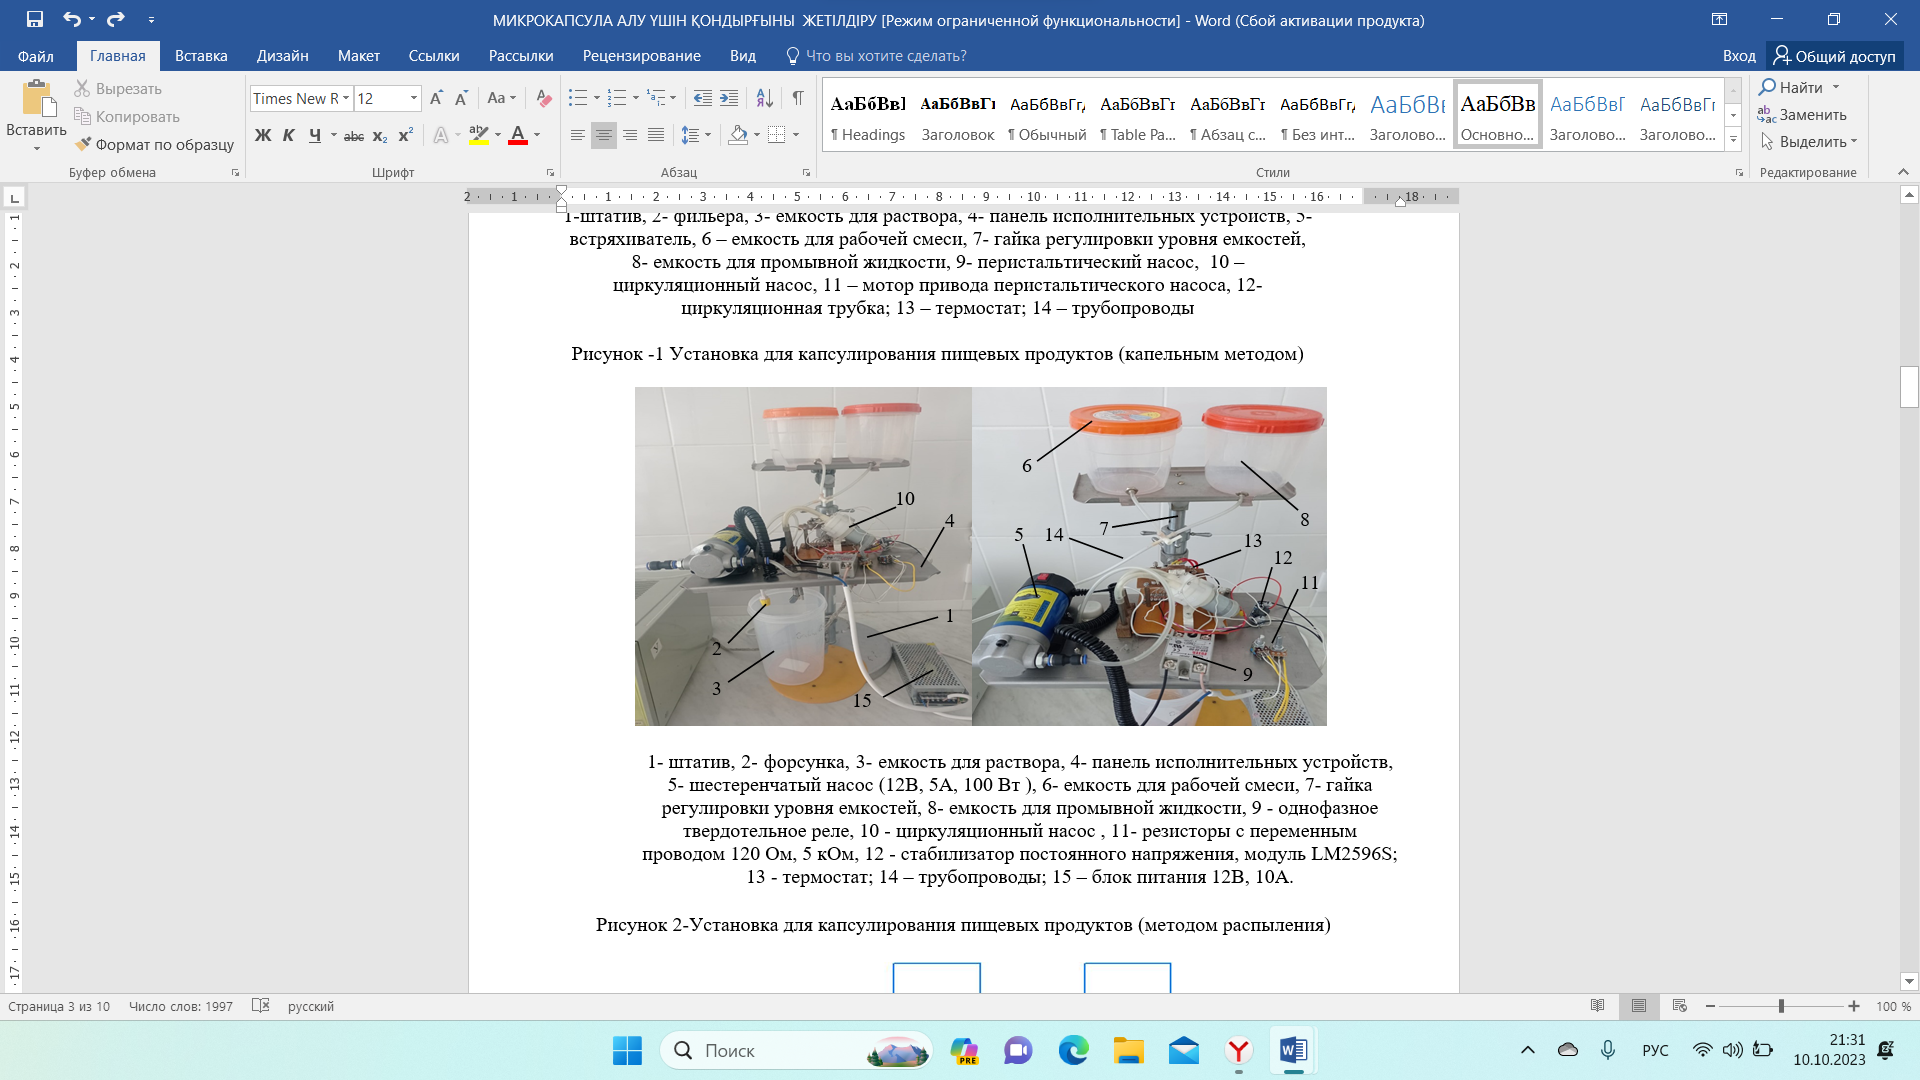
\includegraphics[width=0.8\textwidth]{assets/310}
	\caption*{\emph{1- штатив, 2- форсунка, 3- емкость для раствора, 4- панель
	исполнительных устройств, 5- шестеренчатый насос (12 В, 5 А, 100 Вт ), 6
	- емкость для рабочей смеси, 7- гайка регулировки уровня емкостей, 8-
	емкость для промывной жидкости, 9 - однофазное твердотельное реле, 10 -
	циркуляционный насос , 11- переменные резисторы для грубой и тонкой
	регулировки частоты вращения шестеренчатого насоса , 12 - стабилизатор
	постоянного напряжения, модуль LM2596S; 13 - термостат; 14 --
	трубопроводы; 15 -- блок питания 24 В, 20 А}.

	{Рис. 1 - Установка для капсулирования пробиотиков (методом
распыления)}}
\end{figure}





Была выбрана форсунка с выходным отверстием d=
1,2×10\textsuperscript{-3}м, как наиболее оптимальная и по
производительности, и по качесту получаемых капсул. Для подбора
оптимального процентного соотношения альгината натрия 0,5\%, 0,8\%, 1\%.
Эксперименты проводились при температурах гелеобразующей смеси от 20 до
50 ℃.

В качестве водного раствора гелеобразующей смеси использовали раствор с
добавлением альгината натрия. Раствор получили следующим образом: в воде
(60 \textsuperscript{о}С) растворили альгинат натрия в количестве 1 \%
от общего количества взятой воды. Мерный стакан с водным раствором
альгинат натрия помещается на электромагнитную мешалку с подогревом и
раствор перемешивается до полного растворения альгинат натрия.
Температура подогрева выставляется 60 \textsuperscript{о}С, так как при
температуре ниже 60 \textsuperscript{о}С альгинат натрия плохо
растворяется, а при температуре выше 60 \textsuperscript{о}С альгинат
натрия начинает комковаться. После растворения альгината натрия смесь
охладили до температуры 40°С {[}10, с.2{]}.

В полученную смесь внесли навеску штамма пропионовокислых бактерий
Propionibacterium freudenreichii. В качестве формообразующей смеси
готовится 2\% раствор хлорида кальция. Для этого берется 98 мл
дистиллированной воды и добавляется 2 грамма хлорида кальция. После
растворения хлорида кальция формообразующая смесь готова.

Технологическую схему установки, показана на рисунке 2 {[}11, с.1{]}. В
емкость 1 для рабочей смеси заливается водный раствор гелеобразующей
смеси (1\% альгината натрия). В емкость 2 заливается промывочная
жидкость для промывки системы после выполнения работы.

\begin{figure}[H]
	\centering
	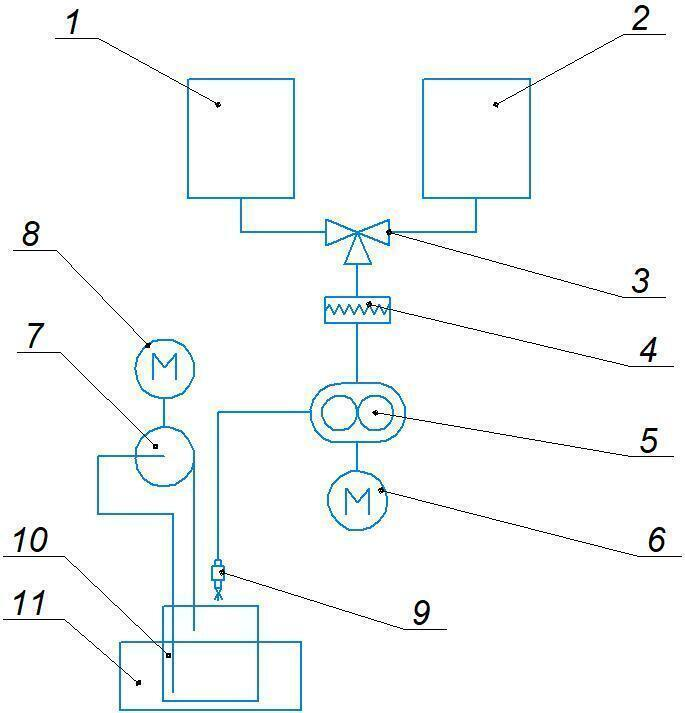
\includegraphics[width=0.8\textwidth]{assets/311}
	\caption*{\emph{1 -- емкость для рабочей смеси; 2 -- емкость для промывной
	жидкости; 3 -- вентиль-переключатель; 4 -- термостат; 5 --}
	\emph{шестеренчатый насос; 6 -- мотор привода шестеренчатого насоса; 7
	--} \emph{циркуляционный насос; 8 -- мотор привода циркуляционного
	насоса; 9 -- форсунка; 10 -- емкость для формообразующего раствора; 11
	-- емкость для охлаждения (льда)}
	
	{\bfseries Рис. 2 - Технологическая схема установки для капсулирования}}
\end{figure}



С помощью вентиля - переключателя 3 раствор из емкостей 1 подается в
общую систему. Термостат 4 предназначен для поддержания температуры
жидкости в системе на должном уровне. (40 град).

Шестеренчатый насос 5 подает жидкость в форсунку 9, где происходит
распыление. Микрокапсулы образуются в формообразующей жидкости,
представляющий из себя хлорид кальция, за счет химического
преобразования альгината натрия в альгинат кальция при реагировании
альгината натрия с формообразующей жидкостью. Для охлаждения
формообразующей жидкости емкость 10 помещается в емкость со льдом 11.
После получения микрокапсул проводится отделение капсул от
формообразующей жидкости с помощью фильтрующей сетки (на схеме не
указано, т.к. не входит в состав оборудования) {[}10, с.3; 11, с.3{]}.

Определение вязкости водного раствора гелеобразующей смеси. Как
известно, аналоговые вискозиметры с круговой шкалой являются простыми и
удобными в использовании.

Для проведения измерений вязкости, необходимо зафиксировать основное
рабочее тело вискозиметра на вертикальной цилиндрической штанге. В
корпусе вискозиметра, на выходной вал электродвигателя крепится ротор.
Частота вращения регулятора скорости вращения ротора находится в
пределах от 0 до 100 об/мин.

Методология измерения вязкости состоит из нескольких этапов:

Подготовка пробы, путем размещения ее в химической посуде объемом не
менее 600 мл. Выбор подходящего наконечника ротора и его крепление к
выходному валу ротора. Тип необходимого наконечника определяется а
зависимости от вязкости исследуемой жидкости. С целью проведения
измерений в гелеобразных средах, необходимо использовать наконечник
ротора № 4. Использование других типов наконечников, не соответствующих
типу измеряемой смеси, не даст адекватных результатов измерения. 1.
Помещение рабочего элемента в исследуемую пробу. 2. Включение
вискозиметра. 3. Определение необходимой скорости вращения ротора. 4.
Стабилизация показаний (время стабилизации определяется в среднем после
5 оборотов ротора и находится в прямой зависимости от скорости вращения
и характеристик исследуемой жидкости). 5. Снятие показаний с круговой
шкалы.

В соответствии с номером использованного ротора и скоростью вращения,
определяется табличный коэффициент, на который нужно умножить показания
с круговой шкалы вискозиметра. Если необходимо получить данные в мПа-с,
данные с круговой шкалы вискозиметра необходимо умножить на фактор F
(табличный коэффициент), соответствующий определенному ротору {[}10,
с.4{]}.

{\bfseries Результаты и обсуждения.} Для выявления изменения значений
экспериментальных данных, построены графики зависимости вязкости
гелеобразующей смеси от температуры раствора и частоты вращения ротора
вискозиметра. Показано на рисунке 3,4,5,6. Диапазон исследуемых
температур был выбран от 20 до 50 ºС, так как при температурах ниже 20
ºС водный раствор гелеобразующей смеси загустевает и соответственно
перестает течь через форсунку, а при температурах выше 50 ºС пробиотики
погибают.

При определении вязкости в вискозиметре Брукфильда постоянный режим
выходит после частоты вращения ротора от 0,333 с\textsuperscript{-1} до
0,833 с\textsuperscript{-1}.

\begin{figure}[H]
	\centering
	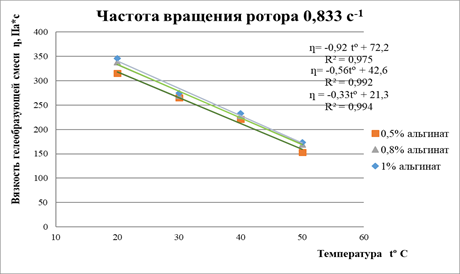
\includegraphics[width=0.8\textwidth]{assets/312}
	\caption*{Рис.3 -Зависимость вязкости гелеобразующей смеси от температуры
	раствора и количества альгината натрия частоты вращения ротора 0,833
	с\textsuperscript{- 1}}
\end{figure}


\begin{figure}[H]
	\centering
	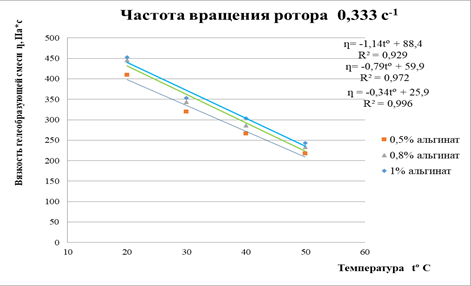
\includegraphics[width=0.8\textwidth]{assets/313}
	\caption*{Рис. 4 - Зависимость вязкости гелеобразующей смеси от
	температуры раствора и количества альгината натрия частоты вращения ротора 0,333
	с\textsuperscript{- 1}}
\end{figure}


Показано на рисунке 3 - 4 с раствором альгината натрия, на графике
зависимости вязкости гелеобразующей смеси от температуры раствора при
частоте вращения ротора вискозиметра 0,833 с\textsuperscript{- 1} и
0,333 с\textsuperscript{- 1} в экспериментальной установке для получения
капсул, вязкость значительно увеличивается при понижении температуры, а
по мере увеличения концентрации вязкость гелеобразующей смеси
увеличивается.

\begin{figure}[H]
	\centering
	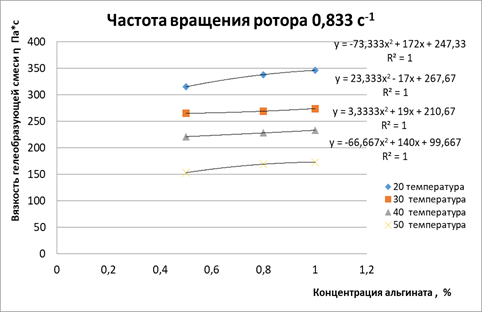
\includegraphics[width=0.8\textwidth]{assets/314}
	\caption*{ Рис. 5 - Зависимость вязкости гелеобразующей смеси от
	концентрации раствора альгината натрия при различных температурах}
\end{figure}



\begin{figure}[H]
	\centering
	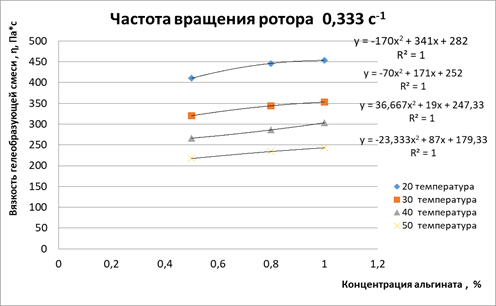
\includegraphics[width=0.8\textwidth]{assets/315}
	\caption*{Рис. 6 - Зависимость вязкости гелеобразующей смеси от
	концентрации раствора альгината натрия при различных температурах}
\end{figure}



Зависимость вязкости гелеобразующей смеси от концентрации раствора
альгината натрия при различных температурах, из графиков на рисунке 5 -
6 видно, что при температурах 40 и 50 С° величина вязкости незначительно
изменяется для частоты вращения ротора, но для предотвращения гибели
пробиотических микроорганизмов не рекомендуется использовать температуру
выше 50 С°\emph{{\bfseries .}} Исходя из всего этого, наиболее подходящая
температура для использования раствора составляет 40 С°.

В условиях напряженного состояния, при приложении силы, поведение
неньютоновских жидкостей характеризуется напряжением, геометрическими
размерами канала и скоростью истечения жидкости {[}12{]}.

Модели, которые характеризуются упругостью и вязкостью, составляют
совокупность тел механической модели реологического тела продукта. Их
деформационное поведение описывается реологическими уравнениями {[}12,
с.14{]}.

Гелеобразное сырье при нагнетании давления с помощью шестеренчатого
насоса испытывает мгновенно-упругую деформацию (G) и в дальнейшем, при
напряжении превышающем предел текучести (θт), вязкопластическую (η)
деформацию. Под действием давления и испытываемых деформаций,
гелеобразное сырье попадает в форсунку, разбрызгивается, в дальнейшем
образует микрокапсулы.

Используя механические модели Бингама {[}12, с.18{]}, Шведова {[}13{]},
Шоффильда-Скоттблера {[}14{]}, Пелега {[}15{]} и проведения обоснования
с целью описания поведения гелеобразного сырья при механическом
воздействии, можно получить механическую модель реологического тела.
Данная модель реологического тела представляет собой модель Бюргерса
{[}16{]} в соответствии с рисунком 7 {[}10, с.9; 12, с.20{]}, т.е.
последовательную механическую модель вязко - упругого релаксирующего
тела Максвелла и вязко - упругого тела Кельвина -- Фойгта для
гелеобразной среды.

Таким образом, общая деформация гелеобразного сырья для данной модели
представляет собой сумму деформаций тела Максвелла и элемента,
моделирующего поведение сырья, которое отражает явление упругого
последствия, представляющее собой изменение упругой деформации с
течением времени


	\emph{∆γ= ∆γ\textsubscript{М} + ∆γ\textsubscript{К} }    (1)


где, \emph{∆γ\textsubscript{М}}-- деформация модели Максвелла;

\emph{∆γ\textsubscript{К}} - деформация модели Кельвина -- Фойгта

\begin{figure}[H]
	\centering
	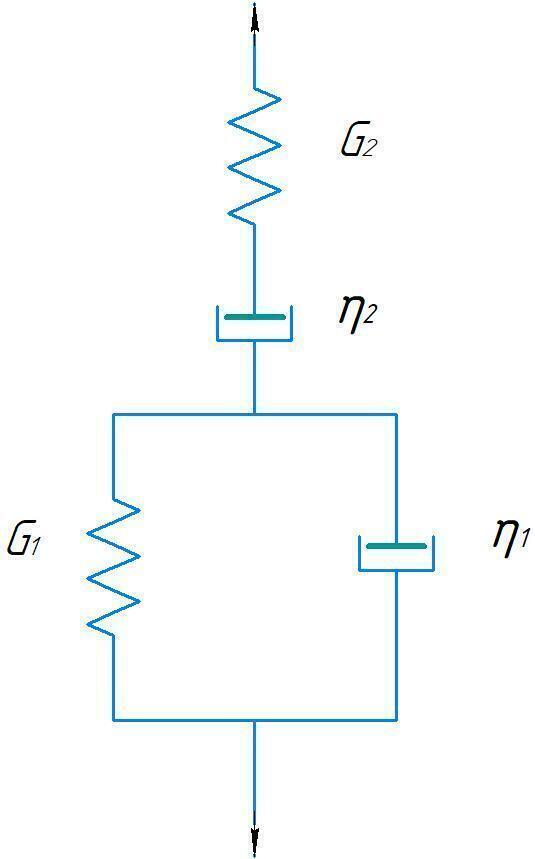
\includegraphics[width=0.2\textwidth]{assets/317}
	\caption*{\emph{G\textsubscript{1} - модуль мгновенной эластичной деформации, Па;
	G\textsubscript{2} - модуль замедленной упругой деформации, Па;
	η\textsubscript{1} -- ньютоновская вязкость, Па·с; η\textsubscript{2}
	--пластическая вязкость при сдвиге, Па·с}
	
	{\bfseries Рис. 7 -- Механическая модель Бюргерса}}
\end{figure}



Производная по времени от левой и правой частей уравнения (1) имеет вид:

% \begin{longtable}[]{@{}
%   >{\raggedright\arraybackslash}p{(\columnwidth - 2\tabcolsep) * \real{0.8059}}
%   >{\raggedright\arraybackslash}p{(\columnwidth - 2\tabcolsep) * \real{0.1941}}@{}}
% \toprule\noalign{}
% \begin{minipage}[b]{\linewidth}\raggedright
% \begin{figure}[H]
% 	\centering
% 	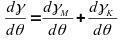
\includegraphics[width=0.8\textwidth]{assets/318}
% 	\caption*{}
% \end{figure}.
% \end{minipage} & \begin{minipage}[b]{\linewidth}\raggedright
% (2)
% \end{minipage} \\
% \midrule\noalign{}
% \endhead
% \bottomrule\noalign{}
% \endlastfoot
% \end{longtable}

Реологическое уравнение модели Максвелла {[}12, с.17{]} определяет
величину \begin{figure}[H]
	\centering
	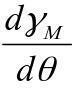
\includegraphics[width=0.8\textwidth]{assets/319}
	\caption*{}
\end{figure}:

% \begin{longtable}[]{@{}
%   >{\raggedright\arraybackslash}p{(\columnwidth - 2\tabcolsep) * \real{0.7850}}
%   >{\raggedright\arraybackslash}p{(\columnwidth - 2\tabcolsep) * \real{0.2150}}@{}}
% \toprule\noalign{}
% \begin{minipage}[b]{\linewidth}\raggedright
% \begin{figure}[H]
% 	\centering
% 	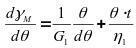
\includegraphics[width=0.8\textwidth]{assets/320}
% 	\caption*{}
% \end{figure}
% \end{minipage} & \begin{minipage}[b]{\linewidth}\raggedright
% (3)
% \end{minipage} \\
% \midrule\noalign{}
% \endhead
% \bottomrule\noalign{}
% \endlastfoot
% \end{longtable}

Величина \begin{figure}[H]
	\centering
	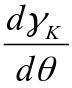
\includegraphics[width=0.8\textwidth]{assets/321}
	\caption*{}
\end{figure} определяется реологическим
уравнением модели Кельвина - Фойгта {[}17, 12, с.16{]}:

\begin{longtable}[]{@{}
  >{\raggedright\arraybackslash}p{(\columnwidth - 2\tabcolsep) * \real{0.8472}}
  >{\raggedright\arraybackslash}p{(\columnwidth - 2\tabcolsep) * \real{0.1528}}@{}}
\toprule\noalign{}
\begin{minipage}[b]{\linewidth}\raggedright
\[\frac{d\gamma_{K}}{d\theta} = \left( \frac{\theta}{G_{2} \cdot d\theta} \right) \cdot \lbrack 1 - e^{( - G_{2} \cdot t/\eta_{2})}\rbrack\]
\end{minipage} & \begin{minipage}[b]{\linewidth}\raggedright
(4)
\end{minipage} \\
\midrule\noalign{}
\endhead
\bottomrule\noalign{}
\endlastfoot
\end{longtable}

Подставляя это значение в выражение (2) получим уравнение Бюргерса для
гелеобразного сырья {[}12, с.19{]}:

\begin{longtable}[]{@{}
  >{\raggedright\arraybackslash}p{(\columnwidth - 2\tabcolsep) * \real{0.8422}}
  >{\raggedright\arraybackslash}p{(\columnwidth - 2\tabcolsep) * \real{0.1578}}@{}}
\toprule\noalign{}
\begin{minipage}[b]{\linewidth}\raggedright
\[\dot{\gamma} = \frac{\theta}{G_{1}} + \frac{\theta \cdot t}{\eta_{1}} + (\frac{\theta}{G_{2}}) \cdot \lbrack 1 - e^{( - G_{2} \cdot t/\eta_{2})}\rbrack\]
\end{minipage} & \begin{minipage}[b]{\linewidth}\raggedright
(5)
\end{minipage} \\
\midrule\noalign{}
\endhead
\bottomrule\noalign{}
\endlastfoot
\end{longtable}

где: \begin{figure}[H]
	\centering
	
\includegraphics[width=0.8\textwidth]{assets/322}
	\caption*{}
\end{figure} - градиент скорости,
с\textsuperscript{-1}; \emph{G\textsubscript{1}} - модуль мгновенной
эластичной деформации, Па; \emph{G\textsubscript{2}} - модуль
замедленной упругой деформации, Па; \emph{η\textsubscript{1}} --
ньютоновская вязкость, Па·с; \emph{η\textsubscript{2}} --пластическая
вязкость при сдвиге, Па·с; \emph{θ} -- касательное напряжение, Па;
\emph{t} -- время, с.

Полученная математическая модель с достаточной точностью позволит
описать процесс истечения гелеобразной жидкости из форсунки для
экспериментальной установки. Представленная модель применима к
установкам с подобным принципом действия, вне зависимости от их
габаритов {[}10, с.10{]}.

Для получения микрокапсул эксперимент проводили с применением форсунки с
выходным отверстием d= 1,2×10\textsuperscript{-3}м {[}10, с.6-7{]}.

\begin{figure}[H]
	\centering
	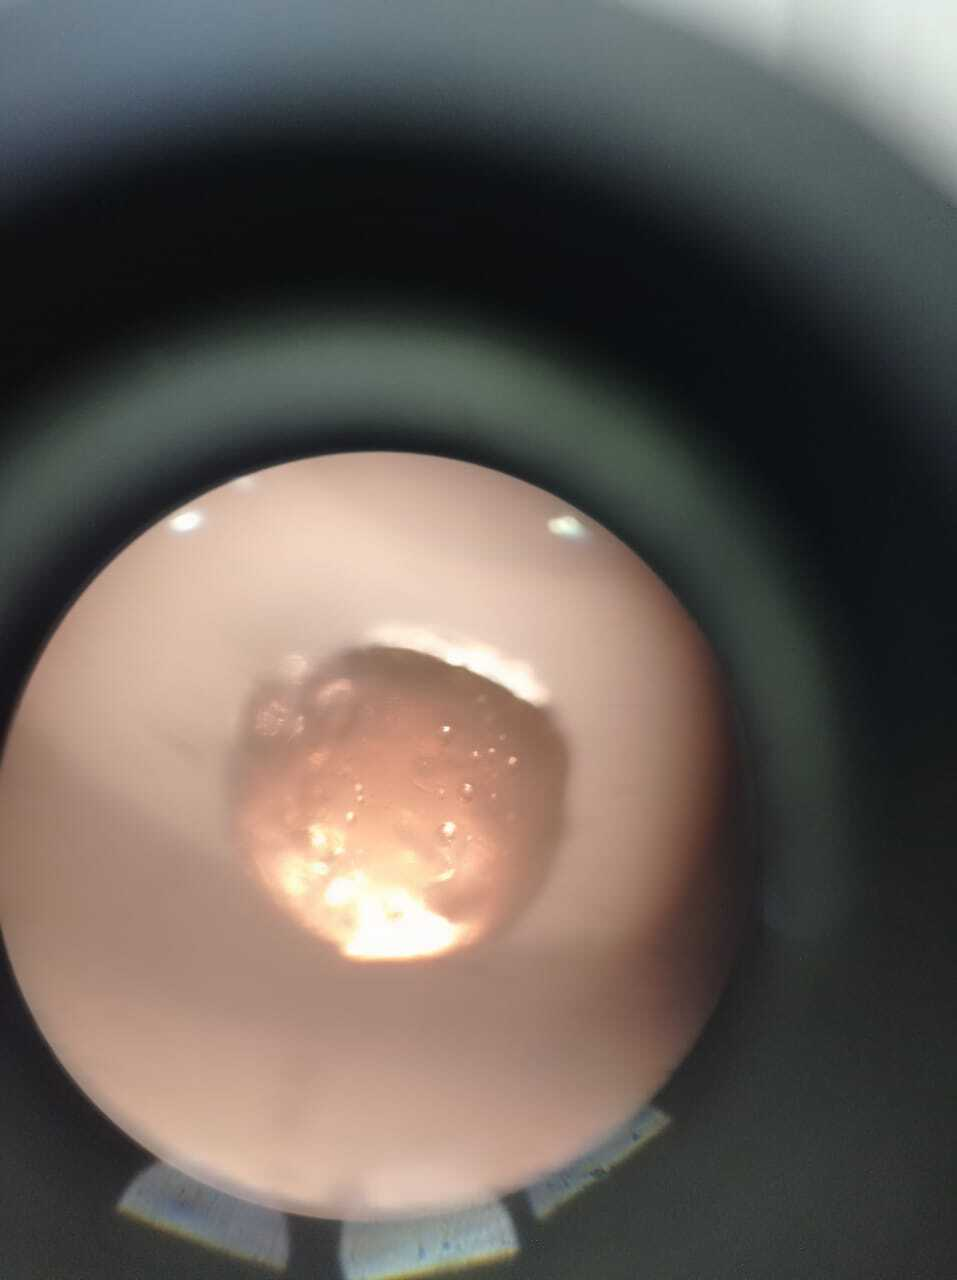
\includegraphics[width=0.8\textwidth]{assets/323}
	\caption*{Рис. 8- Микрокапсула 0,5\% альгинат натрия}
\end{figure}



При концентрации 0,5\% альгината натрия полученные капсулы имеют
округлую, но не всегда правильную форму и однородную структуру, мягкую
консистенцию, легко разрушаются при физическом воздействии и имеют
средний размер 1,2 · 10 \textsuperscript{-3}м.

\begin{figure}[H]
	\centering
	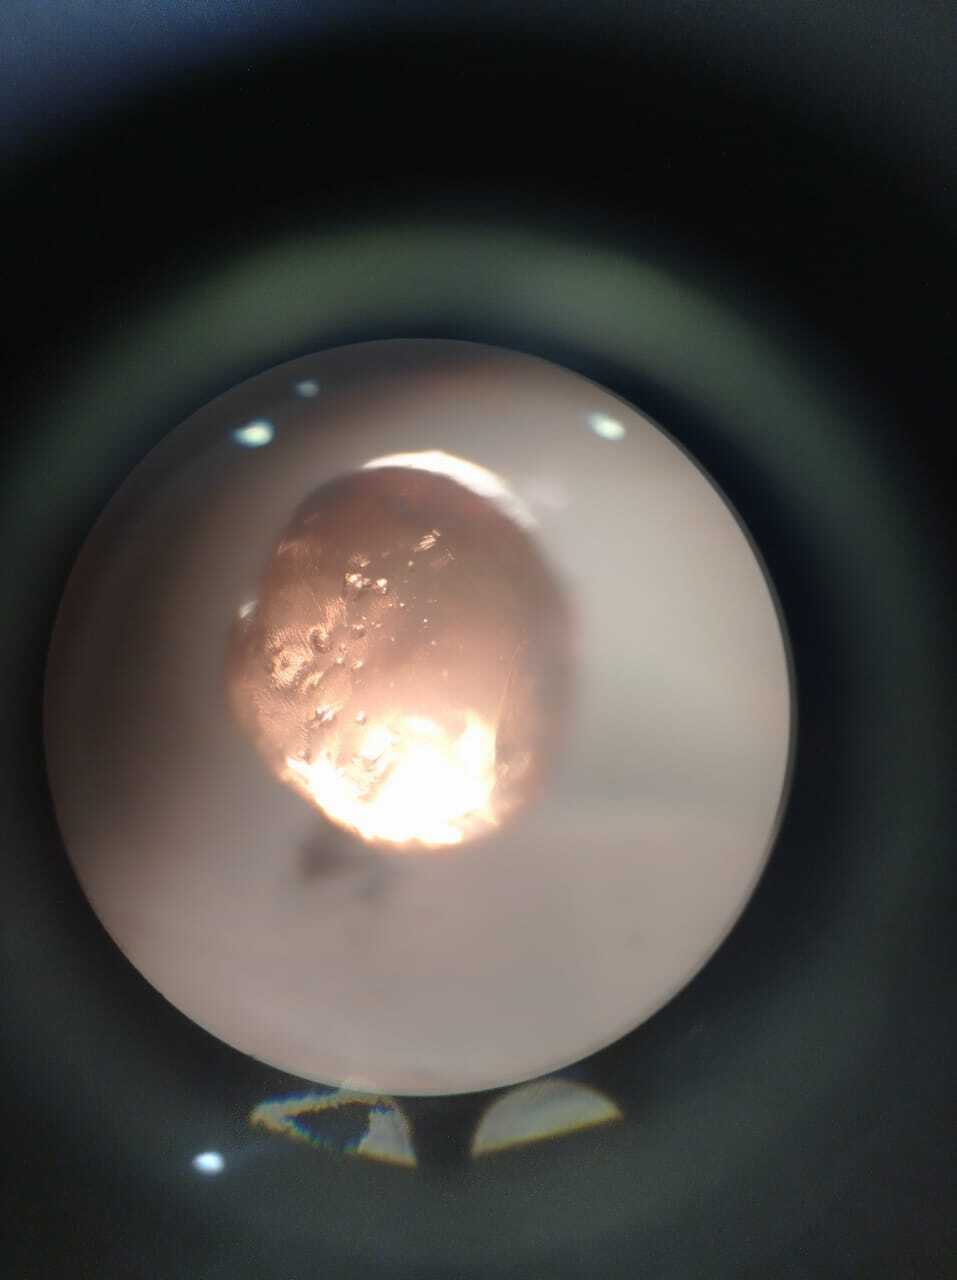
\includegraphics[width=0.8\textwidth]{assets/324}
	\caption*{Рис. 9 -Микрокапсула 0,8\% альгинат натрия}
\end{figure}



При концентрации 0,8\% альгината натрия полученные капсулы имеют
округлую форму и однородную структуру, мягкую консистенцию, легко
разрушаются при физическом воздействии и имеют средний размер
1,3×10\textsuperscript{-3}м.

\begin{figure}[H]
	\centering
	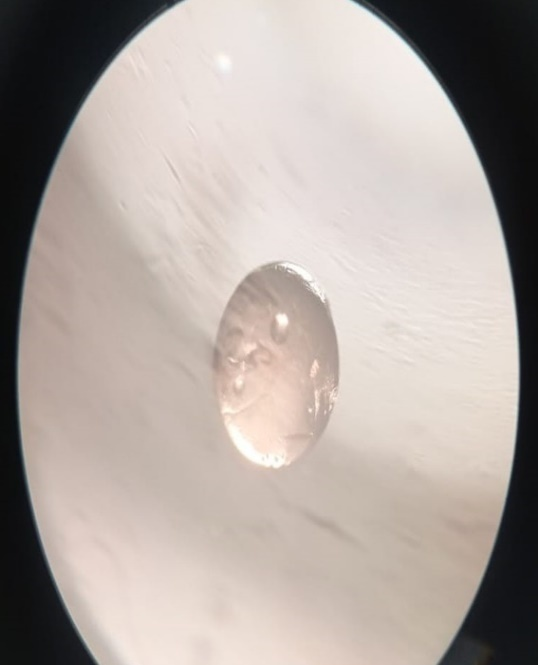
\includegraphics[width=0.8\textwidth]{assets/325}
	\caption*{Рис.10- Микрокапсула 1 \% альгинат натрия}
\end{figure}



При концентрации 1\% альгината натрия полученные капсулы имеют округлую
форму и однородную структуру, мягкие на ощупь, но устойчивые при
физическом воздействии и имеют средний размер составил
1,4×10\textsuperscript{-3}м

Проводя анализ капсул, можно сделать вывод: что наиболее оптимальным
вариантом является состав раствора, содержащий 1\% альгинат натрия.
Капсулы, изготовленные из этого раствора, имеют красивую округлую форму,
одинаковый размер, мягкую консистенцию, но устойчивую для физического
воздействия.

{\bfseries Выводы.} В настоящее время микрокапсулы стали применяться в
сельском хозяйстве, фармацевтике в различных отраслях промышленности.
При проведении экспериментов использовали в качестве распылителя
пластиковую форсунку с выходным диаметром d=
1,2×10\textsuperscript{-3}м. Для экспериментов готовили растворы в
концентрациях 0,5\%, 0,8\%, 1\% альгината. Для подбора оптимальных
размеров капсул построены графики зависимости вязкости гелеобразующей
смеси от температуры раствора и скорости вращения вискозиметра ротора.
Исследуемый диапазон температур выбирался от 20 до 50 ºС. Для
определения изменения значений экспериментальных данных построены
графики зависимости вязкости гелеобразующей смеси от температуры
раствора и концентрации раствора при различных температурах.

В конечном итоге, получили округлые капсулы, содержащие пробиотик
Propionibacterium freudenreichii, которые могут быть использованы в
дальнейших технологических процессах при получении пищевых продуктов
лечебно-профилактического действия или при получении фармокологических
препаратов.



\begin{center}
	{\bfseries Литература}
	\end{center}
\begin{noparindent}

1. Жумадилова Г. А. Исследование процесса инкапсулирования пробиотиков с
целью создания обору-дования: дисс \ldots{} PhD - 6D072400. - Семей: НАО
«Университет имени Шакарима города Семей», 2020.- 131с.

2. Какимов А.К., Ибрагимов Н.К., Муратбаев А.М., Джумажанова М.М.,
Жумадилова Г.А. Инкапсу-лирование в пищевой промышлености // Пищевые
инновации и биотехнологии: сборник тезисов VII Международной научной
конференции студентов, аспирантов и молодых ученых. Т. 1. Технологии
пищевых производств, качество и безопасность / под общ. ред. А. Ю.
Просекова: ФГБОУ ВО \\«Кемеровский государственный университет».-Кемерово,
2019. - С. 153-154.

3. A.Kakimov, Kakimova Zh., Mirasheva G., Bepeyeva A., Toleubekova S.,
Jumazhanova M., Zhumadilova G., Yessimbekov Zh. Amino Acid Composition
of Sour-milk Drink with Encapsulated Probiotics // Annual Research \&
Review in Biology.- 2017.- Vol.18(1).- P.1-7. DOI 10.9734/ARRB/2017/36079

4. Какимов А.К., Какимова Ж.Х., Бепеева А.Е., Джумажанова М.М,
Жумадилова Г.А. Безопасность, функциональные и технологические свойства
пробиотических бактерий // Сборник научных трудов, посвященный 60-летию
отдела сибниис федеральное государственное бюджетное научное учреждение
Фанца. Актуальные проблемы техники и технологии переработки молока,
Барнаул: 2018.- C.-162-165

5. Муратбаев А. М. Капсулаланған биологиялық белсенді қоспаларды
қолданып өндірілген,тамақ өнімдерінің қауіпсіздігін қамтамасыз етудің
тәжірибелік аспектілері: дисс. ...РhD - 6D073500. -- Семей: Семей
қаласының Шәкәрім атындағы университеті, 2021. -- 169 с.

6. Burgain J., Gaiani C., Linder M., Scher J. Encapsulation of probiotic
living cells: From laboratory scale to industrial applications// Journal
of Food Engineering.-2011.-Vol.104(4) - Р.467--483. DOI
10.1016/j.\\jfoodeng.2010.12.031

7. Rowley J.A., Madlambayan G., Mooney D.J. Alginate hydrogels as
synthetic extracellular matrix \\materials//Biomaterials.- 1999.-Vol. 20
(1).- Р. 45- 53. DOI~10.1016/s0142-9612(98)00107-0

8. Krasaekoopt W., Bhandari B., Deeth H. Evaluation of encapsulation
techniques of probiotics for yoghurt //International Dairy
Journal.-2003.- Vol.13(1).- Р. 3--13. DOI 10.1016/S0958-6946(02)00155-3

9. Cook M.T., Tzortzis G., Charalampopoulos D.,. Khutoryanskiy V. V.
Microencapsulation of probiotics for gastrointestinal delivery. Review//
Journal of Controlled Release. - 2012.- Vol.162 - Р. 56 - 67. DOI
10.1016/j.jconrel.2012.06.003

10. M. Tashybayeva, A. Kakimov, N. Ibragimov, G. Zhumadilova, А.
Muratbayev, M. Jumazhanova, B. Idyryshev, Z. Kapshakbayeva, A. Bepeyeva
Optimization of encapsulation parameters for sodium alginate capsules: A
study on the effect of temperature and gear pump rotation speed on
capsule production and quality// Journal of Food Process Engineering.-
2024- Vol.47(7) DOI 10.1111/jfpe.14687

11. Ташыбаева М.М., Какимов А.К., Майоров А.А., Ибрагимов Н.К.,
Джумажанова М.М., \\Жумадилова Г.А., Муратбаев А.М., Бакиева А.Б.,
Дукенбаев Д.К. Капсулаған өнімдерді өндіруге арналған қондырғы / ҚР
пайдалы модельге патенті № 9093, 03.05.2024ж.

12. Мачихин Ю.А., Мачихин С.А. Инженерная реология пищевых продуктов. -
М.: Легкая и пищевая промышленность.- 1981.-215 с.

13. Sсhоfie1d R. K., Scott Blair G. W. The relationschip between
viscosity, elasticity and plastics strenght of a soft material as
illustrated by some mechanical properties of flour dough. --- Proc. Roy.
Soc.-1932. - P. 707- 718.DOI 10.1098/pspa.1933.0038

14. Scott Blair G. W. Psycho-rheology. --- J. Texture Studies, 1.-
1970.- P. 231

15. Реleg M. Contact and fracture elements as components of the
rheolo-gical memory of solid foods. --- J. Texture Studies 8, 1977. - P.
39 - 48. DOI~10.1111/j.1745-4603.1977.tb01164.x

16. Шрам Г. Основы практической реологии и реометрии -- М.: Колос С,
2003. -- 312 с. ISBN 5-9532-0234-2

17.Горбатов А.В., Реология мясных и молочных продуктов. -- М.: Пищевая
промышленность, 1979. -- 383 с.

\end{noparindent}

\begin{center}
{\bfseries References}
\end{center}

\begin{noparindent}

1. Zhumadilova G. A. Issledovanie processa inkapsulirovanija probiotikov
s cel\textquotesingle ju sozdanija oborudovanija: diss \ldots{} PhD -
6D072400. - Semej: NAO «Universitet imeni Shakarima goroda Semej»,
2020.- 131s. {[}in Russian{]}

2. Kakimov A.K., Ibragimov N.K., Muratbaev A.M., Dzhumazhanova M.M.,
Zhumadilova G.A. \\Inkapsulirovanie v pishhevoj promyshlenosti //
Pishhevye innovacii i biotehnologii: sbornik tezisov VII Mezhdunarodnoj
nauchnoj konferencii studentov, aspirantov i molodyh uchenyh. T. 1
Tehnologii pishhevyh proizvodstv, kachestvo i
bezopasnost\textquotesingle{} / pod obshh. red. A. Ju. Prosekova: FGBOU
VO «Kemerovskij gosudarstvennyj universitet».-Kemerovo, 2019. - S.
153-154{\bfseries .} {[}in Russian{]}

3. A.Kakimov, Kakimova Zh., Mirasheva G., Bepeyeva A., Toleubekova S.,
Jumazhanova M., Zhumadilova G., Yessimbekov Zh. Amino Acid Composition
of Sour-milk Drink with Encapsulated Probiotics // Annual Research \&
Review in Biology.- 2017.- Vol.18(1).- P.1-7. DOI 10.9734/ARRB/2017/36079

4. Kakimov A.K., Kakimova Zh.H., Bepeeva A.E., Dzhumazhanova M.M,
Zhumadilova G.A. Bezopasnost\textquotesingle,
funkcional\textquotesingle nye i tehnologicheskie svojstva
probioticheskih bakterij // Sbornik nauchnyh trudov,\\ posvjashhennyj
60-letiju otdela sibniis federal\textquotesingle noe gosudarstvennoe
bjudzhetnoe nauchnoe uchrezhdenie Fanca. Aktual\textquotesingle nye
problemy tehniki i tehnologii pererabotki moloka, Barnaul: 2018.-
C.-162-165. {[}un Kazakh{]}

5. Muratbaev A. M. Kapsulalanғan biologijalyқ belsendі қospalardy
қoldanyp өndіrіlgen,tamaқ өnіmderіnің қauіpsіzdіgіn қamtamasyz etudің
tәzhіribelіk aspektіlerі: diss. ...RhD - 6D073500. -Semej: Semej
қalasynyң Shәkәrіm atyndaғy universitetі, 2021. -169 s.

6. Burgain J., Gaiani C., Linder M., Scher J. Encapsulation of probiotic
living cells: From laboratory scale to industrial applications// Journal
of Food Engineering.-2011.-Vol.104(4) - Р.467--483. DOI
10.1016/j.\\jfoodeng.2010.12.031

7. Rowley J.A., Madlambayan G., Mooney D.J. Alginate hydrogels as
synthetic extracellular matrix \\materials//Biomaterials.- 1999.-Vol. 20
(1).- Р. 45- 53. DOI~10.1016/s0142-9612(98)00107-0

8. Krasaekoopt W., Bhandari B., Deeth H. Evaluation of encapsulation
techniques of probiotics for yoghurt //International Dairy
Journal.-2003.- Vol.13(1).- Р. 3--13. DOI 10.1016/S0958-6946(02)00155-3

9. Cook M.T., Tzortzis G., Charalampopoulos D.,. Khutoryanskiy V. V.
Microencapsulation of probiotics for gastrointestinal delivery. Review//
Journal of Controlled Release. - 2012.- Vol.162 - Р. 56 - 67. DOI
10.1016/j.jconrel.2012.06.003

10. M. Tashybayeva, A. Kakimov, N. Ibragimov, G. Zhumadilova, А.
Muratbayev, M. Jumazhanova, B. Idyryshev, Z. Kapshakbayeva, A. Bepeyeva
Optimization of encapsulation parameters for sodium alginate capsules: A
study on the effect of temperature and gear pump rotation speed on
capsule production and quality// Journal of Food Process Engineering.-
2024- Vol.47(7) DOI 10.1111/jfpe.14687

11. Tashybaeva M.M., Kakimov A.K., Majorov A.A., Ibragimov N.K.,
Dzhumazhanova M.M., \\Zhumadilova G.A., Muratbaev A.M., Bakieva A.B.,
Dukenbaev D.K. Kapsulaғan өnіmderdі өndіruge arnalғan қondyrғy / ҚR
pajdaly model\textquotesingle ge patentі № 9093, 03.05.2024zh. {[}in
Russian{]}

12. Machihin Ju.A., Machihin S.A. Inzhenernaja reologija pishhevyh
produktov. - M.: Legkaja i pishhevaja promyshlennost\textquotesingle.-
1981.-215 s. {[}in Russian{]}

13. Sсhоfie1d R. K., Scott Blair G. W. The relationschip between
viscosity, elasticity and plastics strenght of a soft material as
illustrated by some mechanical properties of flour dough. --- Proc. Roy.
Soc.-1932. - P. 707- 718.DOI 10.1098/pspa.1933.0038 {[}in Russian{]}

14. Scott Blair G. W. Psycho-rheology. --- J. Texture Studies, 1.-
1970.- P. 231. {[}in Russian{]}

15. Реleg M. Contact and fracture elements as components of the
rheolo-gical memory of solid foods. --- J. Texture Studies 8, 1977. - P.
39 - 48. DOI~10.1111/j.1745-4603.1977.tb01164.x

16. Shram G. Osnovy prakticheskoj reologii i reometrii -- M.: Kolos S,
2003. -- 312 s.

ISBN 5-9532-0234-2

17.Gorbatov A.V., Reologija mjasnyh i molochnyh produktov. -M.:
Pishhevaja promyshlennost\textquotesingle, 1979. - 383 s.

\end{noparindent}

\emph{{\bfseries Сведения об авторах}}

\begin{noparindent}

Ташыбаева М.М.-докторант, Университет имени Шакарима города Семей,
Казахстан, \\е-mail: marzhan06081990@gmail.com.

Какимов А.К.- доктор технических наук, профессор, Университет имени
Шакарима города Семей, Казахстан, е-mail: bibi.53@mail.ru;

Майоров А.А. - доктор технических наук, профессор ФГБНУ Федеральный
Алтайский научный центр агробиотехнологий, Барнаул, Российская
Федерация, е-mail: maiorov.alex@mail.ru;

Жумадилова Г.А. - PhD, Университет имени Шакарима города Семей,
Казахстан; \\е- mail: zhumadilovaga@mail.ru.

\end{noparindent}

\emph{{\bfseries Information about authors}}

\begin{noparindent}

Tashybayeva M.М{\bfseries .} - doctoral student, Shakarim University of
Semey, Kazakhstan, \\e-mail: marzhan06081990@gmail.com;

Kakimov А.К. -- doctor of technical sciences, Shakarim University of
Semey, Kazakhstan, \\e-mail: bibi.53@mail.ru;

Mayorov A.А. - doctor of technical sciences, professorederal State
Budget Scientific Institution Federal Altai Scientific Center for
Agrobiotechnologies , Barnaul, Russian, e-mail: maiorov.alex@mail.ru;

Zhumadilova G.А.{\bfseries -} PhD, Shakarim University of Semey,
Kazakhstan; e-mail: zhumadilovaga@mail.ru.


\end{noparindent}